\documentclass{article} % A4 paper and 11pt font size

\usepackage[T1]{fontenc} % Use 8-bit encoding that has 256 glyphs
\usepackage[danish]{babel} % English language/hyphenation
\usepackage{amsmath,amsfonts,amsthm} % Math packages

\usepackage{sectsty} % Allows customizing section commands
\usepackage{tikz}
\setlength{\headheight}{13.6pt} % Customize the height of the header

\usepackage{commath}
\setlength\parindent{0pt} % Removes all indentation from paragraphs - comment this line for an assignment with lots of text
\usepackage[danish]{babel}
\usepackage[danish]{cleveref}
\usepackage{noter}
%----------------------------------------------------------------------------------------
%   TITLE SECTION
%----------------------------------------------------------------------------------------

\newcommand{\horrule}[1]{\rule{\linewidth}{#1}} % Create horizontal rule command with 1 argument of height

\title{
\normalfont \normalsize
\textsc{Mål og Integral teori} \\ [25pt] % Your university, school and/or department name(s)
\horrule{0.5pt} \\[0.4cm] % Thin top horizontal rule
\huge Aflevering 2 \\ % The assignment title
\horrule{2pt} \\[0.5cm] % Thick bottom horizontal rule
}

\author{Rud V. Faden, Alex Larsen, Markus Bak Hansen, Nemo Bremer, Theis Kehlet} % Your name

\date{\normalsize\today} % Today's date or a custom date
\usepackage{hyperref}

\begin{document}
\maketitle
\section*{Momenter}
\label{sec:title}

\paragraph*{Spørgsmål 1.a}
Først beregner vi \(E(\tilde{X})\). Da \(E(X)=E(Y)=0<\infty\), da kan vi bruge teorem 16.3 in EH.
\begin{align}
E(\tilde{X})=E(aX+bY)=E(aX)+E(bY)=aE(X)+bE(Y)=0
\end{align}
da \(E(X)=E(Y)=0\). Ved symmetri fås at \(E(\tilde{Y})=0\).
\paragraph*{Spørgsmål 1.b}
Variansen af en stokastisk variable er givet ved \(E(X-E(X))^2\). Ved indsætning af \(\tilde{X}\) fås
\begin{align}
	V(\tilde{X}) & = E\left((aX+bY)-E(aX+bY)\right)^2 \\
	           & = E\left((aX+bY)^2\right)-\left(E(aX+bY)\right)^2\label{varians}
\end{align}
Men vi har lige vist at \(E(aX+bY)=0\), så \eqref{varians} reduceres til
\begin{align}
	V(\tilde{X}) & = E\left((aX+bY)^2\right) \\
	           & = E\left(a^{2}X^2+b^2Y^2+2abXY\right) \\
	           & = a^2E(X^2)+b^2E(Y^2)+2abE(XY)
\end{align}
Men da \(E(XY)=0\), fås
\begin{align}
    V(\tilde{X}) &= a^2E(X^2)+b^2E(Y^2) \label{var_x}
\end{align}
Vi ser nu at \(V(X)=E(X^2)=1\) og at \(V(Y)=E(Y^2)=1\), så \cref{var_x} kan skrives som
\begin{align}
     V(\tilde{X}) &= a^2+b^2 \label{var_x_2}
\end{align}
Ved symmetri fås at
\begin{align}
    V(\tilde{Y}) &= c^2+d^2 \label{var_y}
\end{align}
\paragraph*{Spørgsmål 1.c}
Vi kan skrive \cref{var_x_2} og \cref{var_y} som matrix
\begin{align}
O^TO=OO^T=
	\begin{pmatrix}
  a & b \\
  c & d
	\end{pmatrix}
	\begin{pmatrix}
  a & c \\
  b & d
	\end{pmatrix}
	=
	\begin{pmatrix}
	a^2 + b^2 & ab+cd \\
	ab+cd & c^2 + d^2
	\end{pmatrix}
  =I=V
  \begin{pmatrix}
  \tilde{X} \\
  \tilde{Y}
  \end{pmatrix}
\end{align}


\paragraph*{Spørgsmål 2.a}
Vi skal nu vise, under hvilken betingelser på \(O\), at \(\tilde{X}\) og \(\tilde{Y}\) er ukorreleret. To stokastiske variable er ukorreleret hvis \(Cov(\tilde{X},\tilde{Y})=0\). Dette kan også skrive med forventningsoperatoren som
\begin{align}
   E((\tilde{X}-E\tilde{Y})(\tilde{Y}-E\tilde{Y}))=E\tilde{X}\tilde{Y}-E\tilde{X}E\tilde{Y}=0
\end{align}

Men da vi har at \(E\tilde{X}=E\tilde{Y}=0\) fra forrige opgave, kan vi skrive kovariansen som \(E\tilde{X}\tilde{Y}\)
\begin{align}
	E\left(\left[aX+bY\right]\left[cX+dY\right]\right) &=0 \\
	acE(X^2)+bdE(Y^2)+adE(XY)+bcE(XY)                  &=0 \label{tilde_var}
\end{align}
Men da \(E(XY)=0\) og \(V(X)=V(Y)=E(X^2)=E(Y^2)=1\), ser vi at \cref{tilde_var} kan skrives som
\begin{align}
    ac+bd=0 \label{opg:2a}
\end{align}
Hvilket altid gælder, hvis \(O\) er en ortogonal matrix.
\paragraph{Spørgsmål 2.b}
Vi ser at hvis \cref{opg:2a} skal holde, så skal \(bd=-ac\). Dermed kan vi skrive
\begin{align}
    E(acX^2-acY^2) & = 0 \\
    acE(X^2-Y^2) & = 0 \\
\end{align}
Da \(ac\ne 0\), da må vi dividere med \(ac\). Dermed har vi at
\begin{align}
    E(X^2-Y^2)=E(X+Y)(X-Y)=0
\end{align}
og dermed at \(X-Y,X+Y\) er ukorrelert.

\section*{Transformationer} % (fold)
\label{sec:transformationer}
\paragraph*{Spørgsmål 3.a}
Vi ser at \((\R^2,\B_2)\) er en sigma-endelig mål rum. Derfor bruger vi lemma 12.2 i EH til at finde den marginale tæthed af \(g(x,y)\)
\begin{align}
    \int g(x,y)\dif m(y) & = \int f(x)f(y)\dif x\dif y \\
                         & = f(x)\int f(y)\dif y \\
                         & = f(x)\cdot 1 = f(x)
\end{align}
Da \(m\) er et sandsynlighedsmål. Tæthede \(f(y)\) findes på samme måde per symmetri.

\paragraph*{Spørgsmål 3.b}
Vi bruger teorem 12.14 med
\begin{align}
    \nu & = g(x,y) \\
    h(x,y) & =
    \begin{pmatrix}
    	a & b \\
    	c & d
    \end{pmatrix}
    \begin{pmatrix}
     	X \\
     	Y
    \end{pmatrix}\\
    h^{-1} & = \frac{1}{ad-cb}
    \begin{pmatrix}
    	d  & -b \\
    	-c & a
    \end{pmatrix}
    \begin{pmatrix}
     	X \\
     	Y
    \end{pmatrix} \\
    D\left(h^{-1}\right)(x,y) & = h^{-1} \\
    \left|det\left(D\left(h^{-1}\right)(x,y)\right)\right| & = \frac{1}{ad-bc}
\end{align}
Således har vi at
\begin{align}
    \tilde{g}(x,y)=g(\frac{1}{ad-bc}(dx-by),\frac{1}{ad-bc}(-cx+ay))
\end{align}
\paragraph*{Opgave 4.a}
Da \(f(x)\) er standart normalfordelt, så får vi at
\begin{align}
    g(x,y) & = \left(\frac{1}{\sqrt{2\pi}} e^{-x^2/2}\right)\left(\frac{1}{\sqrt{2\pi}} e^{-y^2/2}\right) \\
           & = \frac{1}{2\pi}e^{(-x^2-y^2)/2} \label{opg:4.1a}
\end{align}
Matricen \(O\) er orgothonal, så \(|detO|=1\) og \(\left(\frac{1}{detO}(dx-by)\right)^2=\left(dx-by\right)^2\). Derfor er \(\tilde{g}(x,y)\) givet ved
\begin{align}
   \tilde{g}(x,y) & =  \frac{1}{2\pi}e^{-(dx-by)^2/2-(-cx+ay)^2/2} \\
                  & =  \frac{1}{2\pi}e^{-\left((dx-by)^2+(-cx+ay)^2\right)/2} \\
                  & =  \frac{1}{2\pi}e^{-(d^2+c^2)x^2+(b^2+a^2)y^2/2-(db+ac)xy} \label{opg:4.1}
\end{align}
Men da \(O\) er ortogonal har vi at \((d^2+c^2)=(b^2+a^2)=1\) og \((db+ac)=0\). Derfor kan \cref{opg:4.1} skrives som
\begin{align}
   \tilde{g}(x,y) & =  \frac{1}{2\pi}e^{-(x^2+y^2)/2} = g(x,y)
\end{align}
jf. \cref{opg:4.1a}.
% section transformationer (end)
\section{Karakterisering af normalfordelingen} % (fold)
\label{sec:karaktisering_af_normalfordelingen}
\paragraph*{Opgave 5}
For at vise at
\begin{align}
    f(x)f(y) & = f(0)f(\sqrt{x^2+y^2}) \label{opg:5}
\end{align}
omskriver vi til polar koordinater, således at \(x=r\cos(\theta)\), \(y=r\sin(\theta)\) og \(r=\sqrt{x^2+y^2}\)\@. Således har vi at
\begin{align}
     f(r\cos(\theta))f(r\sin(\theta))=f(\theta)f(r)
 \end{align}
 Opskriver vi i matrix form, har vi
 \begin{align}
     \begin{pmatrix}
     0 \\ \sqrt{x^2+y^2}
     \end{pmatrix}
     =
     \begin{pmatrix}
     0 \\
     r
     \end{pmatrix}
 \end{align}
 Vi ser da, at for en hvilken ortogonal transformation af \(x=r\cos(\theta),y=r\sin(\theta)\), vil det gælde at vinklen mellem \(x\) og \(y\) koordinaterne vil blive bevaret. Derved kan dette også udtrykkes som radius \(r\) gange en konstant. Dermed ser vi at  \cref{opg:5} må holde.

 \begin{figure}[htbp]
 	\centering
 	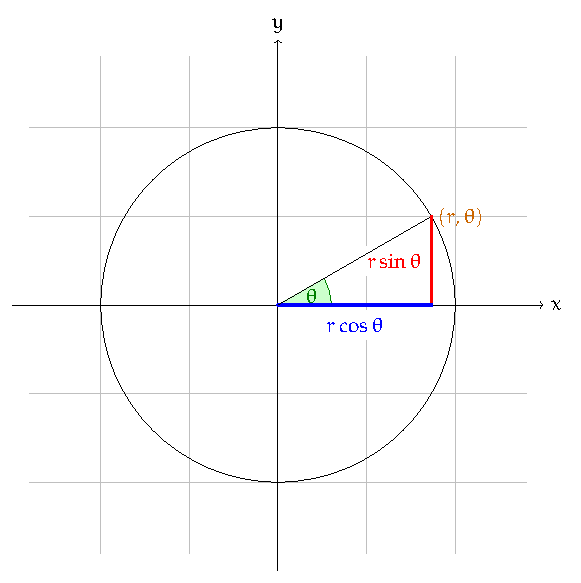
\includegraphics[width=0.95\textwidth]{unitcirle.pdf}
 	\caption{Cirkel}
 	\label{fig:label}
 \end{figure}
\paragraph*{Opgave 6.a}
Vi ser at
\begin{align}
g(x)+g(y)               & = \log\left(\frac{f(x)}{f(0)}\right) + \log\left(\frac{f(y)}{f(0)}\right) \\
                        & = \log(f(x))+\log(f(y))-2\log(f(0))\label{opg:6a}
\end{align}
og at
\begin{align}
g(\sqrt{x^2+y^2})       & = \log\left(\frac{f(\sqrt{x^2+y^2})}{f(0)}\right) \label{eq:36}
\end{align}
Da
\begin{align}
f(x)f(y)                & =f(\sqrt{x^2+y^2})f(0) \\
\frac{f(y)f(x)}{f(0)} & =f(\sqrt{x^2+y^2}) \label{eq:39}
\end{align}
Dermed har vi, ved at indsætte \cref{eq:39} i \cref{eq:36} at
\begin{align}
g(\sqrt{x^2+y^2})       & = \log\left(\frac{f(x)f(y)}{f(0)^2}\right) \\
                        & = \log(f(x))+\log(f(y))-2\log(f(0))\label{opg:6b}
\end{align}
Da \cref{opg:6a} er identisk med \cref{opg:6b} er \(g(x)+g(y)=g(\sqrt{x^2+y^2})\)

\paragraph*{Opgave 6.b}
Cauchy's funktionalligning for \(f\) er
\begin{align}
    f(x)+f(y) & = f(x+y)\\
\end{align}
Heraf følger
\begin{align}
    g(\sqrt{x})       & = f(x)\overbrace{=}^{\text{\makebox[0pt]{Løsning for Cauchy}}} cf =c\sqrt{x^2} \\
    g(\sqrt{x^2+y^2}) & = f(x^2+y^2) = f(x^2)+f(y^2) = g(x)+g(y)
\end{align}
Dermed har vi at løsningen er \(g(x)=cx^2\)
% section karaktisering_af_normalfordelingen (end)
\paragraph*{Spørgsmål 7}
Vi har at
\begin{align}
    g(x)     & = \log{\frac{f(x)}{f(0)}} \\
    e^{g(x)} & = \frac{f(x)}{f(0)}
\end{align}
Indsætter vi løsningen til funktionalligningen fra opgave 6, har vi
\begin{align}
    f(0)e^{cx^2}=f(x) \label{eq:47}
\end{align}
 Da \(f(x)\) er et sandsynlighedsmål, har vi at
 \begin{align}
     \int_{-\infty}^\infty f(x) & = 1 \\
     \int_{-\infty}^\infty f(0)e^{cx^2} = 1
 \end{align}
 Hvis \(c\geq0\), da er \(\int_{-\infty}^\infty f(x)=\infty\). Dermed følger at \(c<0\) skal være opfyldt, for at \(f\) kan være et sandsynlighedsmål.

 For at vise at \(f\sim N(0,(-2c)^{-1})\), bemærker vi først at det er tilfældet hvis
 \begin{align}
      f(x) & = \frac{1}{\sqrt{2\pi(-2c)^{-1}}}e^{-x^2/(2(-2c)^{-1})} \\
      & = \frac{1}{\sqrt{\pi/(-c)}}e^{cx^2} \label{eq:normal}
  \end{align}
og at \(f\) er et sandsynlighed mål, således at
\begin{align}
    \int_{-\infty}^\infty f(0)e^{cx^2}\dif x & = 1 \\
    \int_{-\infty}^\infty e^{cx^2}\dif x & = \frac{1}{f(0)}
\end{align}
Pga. symmetri af funktionen har vi at
\begin{align}
    \int_{0}^\infty e^{cx^2}\dif x & = \frac{1}{2f(0)}
\end{align}
Så
\begin{align}
    \left(\int_{0}^\infty e^{cx^2}\dif x\right)\left(\int_{0}^\infty e^{cy^2}\dif y\right) & = \frac{1}{4f(0)^2} \\
    \int_{0}^\infty e^{c(x^2+y^2)}\dif x \dif y & = \frac{1}{4f(0)^2}
\end{align}
Vi kan evaluere dette integral ved hjælp af polar koordinater.
\begin{align}
    \int_0^{\pi/2}\int_0^{-\infty}e^{cr^2}r\dif r\dif \theta
\end{align}
Ved brug a substitution, med \(u=cr^2\), får vi
\begin{align}
    \int_0^{\pi/2}\frac{1}{2c}\int_0^{-\infty}e^{u}\dif u\dif \theta = \int_0^{\pi/2} -\frac{1}{2c}\dif \theta=\pi(-\frac{1}{4c})
\end{align}
Vi ved derfor at
\begin{align}
    \pi(-\frac{1}{4c}) & = \frac{1}{4f(0)^2} \Leftrightarrow \\
    \pi(-\frac{1}{c}) & = \frac{1}{f(0)^2} \Leftrightarrow \\
    \sqrt{\pi(-\frac{1}{c})} &=  \frac{1}{f(0)} \Leftrightarrow \\
    f(0) &=  \frac{1}{\sqrt{\pi/(-c)}} \Leftrightarrow \label{eq:constant}
\end{align}
Indsætter vi \cref{eq:constant} i \cref{eq:47}, får vi
\begin{align}
    f(x) = \frac{1}{\sqrt{\pi/(-c)}}e^{cx^2}
\end{align}
Hvilket netop er tætheden for \(N(0,(-2c)^{-1})\) jf. \cref{eq:normal}
\end{document}
